\documentclass[color]{tudscrreprt}
\usepackage{caption}
\usepackage{subcaption}
\usepackage[T1]{fontenc}
\usepackage[nottoc,numbib]{tocbibind}
\usepackage{graphicx}
\usepackage{url}
\graphicspath{ {images/} }

\newcommand{\nnewline}{\newline\newline}

\newcommand{\etal}{et al.~}

\newcommand{\etc}{etc.~}

\newcommand{\eg}{e.g.~}

\newcommand{\fig}{Fig.~}

\newbox{\bigpicturebox}
	
\definecolor{Gray}{gray}{0.95}


\let\linksbuendig=\raggedright
\let\raggedright=\relax

\begin{document}

\faculty{Factuly of Computer Science}
\department{Department of Artificial Intelligence}
\institute{Institute of Computer Vision}
\date{\today}
\author{Florian Blume}
\title{%
  Development of a CNN-aided tool to annotate images with 3D models
}
\thesis{Gro\ss er Beleg}
\dateofbirth{12.08.1991}
\placeofbirth{Karlsruhe}
\defensedate{Not yet}
\referee{Eric Brachmann}
\maketitle

\begin{abstract}
Here is an abstract.
\end{abstract}

\tableofcontents

\chapter{Introduction}

About three decades ago, the first minimally invasive surgery was performed. This was a huge step forward, as minimally invasive surgery offers several advantages compared to traditional surgery, such as less pain for the patient and less recovery time needed afterwards \cite{minimallyinvasive}. This kind of operation is more involved for the surgeon, as it is conducted only through a small hole in the otherwise closed abdominal wall. The executing surgeon inserts an endoscope into the patient and only sees the 2D images without any depth. Medical personnel could profit from computers assisting with augmented reality during the surgery. Next to navigation cues and other vital information, the surgical tools could be rendered into the  endoscopic video to compensate the missing depth to some extend and facilitate the operational process. \

This task of annotating images with 3D objects is called 6D pose estimation and is already used and applied in various fields, e.g. robotics, augmented reality, medical imaging, and many more. There exist various ways to recover the 6D poses on an image. 

For well-textured clearly visible objects the task is considered solved. Methods like \cite{dglowe1} by Lowe \etal rely on detecting sparse features, for example keypoints, which are matched against a database that contains the corresponding pose.
Unfortunately, these approaches only work for objects with a strong and also visible texture. After cheap depth sensors like the Xbox Kinect became available, depth-based pose estimation procedures were able to achieve good results on texture-less but unoccluded and non-deformed objects. Many of those methods match the image against a database of templates to recover the pose. 

These techniques have in common that they are non-learning based. This means that there is no learning procedure which learns an object's appearance. Brachman et al. on the other hand used random forests and object coordinates to achieve very good results on the occlusion dataset \cite{brachmann1}. The forests are trained to output for every pixel the 3D location on the object. Using the 2D-3D correspondences, a robust estimate of the object's pose can be computed. Krull et al. \cite{akrull} combine the idea of learning the 3D coordinates representation of an object with the power of the so called \textit{Convolutional Neural Networks (\gls{cnn}s)}. \gls{cnn}s became popular around 2012, after training deeper networks turned out to be achievable in a feasible time on graphics cards. Deep \gls{cnn}s offer outstanding accuracy that beat most traditional computer vision algorithms \cite{ylecun}. A drawback of \gls{cnn}s is their need for training data, which has to be annotated with the desired network output beforehand.

The goal of this work is to create a system that allows users to annotate large datasets, effectively and efficiently. We will introduce a tool that allows to annotate images with the 6D poses of arbitrary objects. To further reduce the time needed to annotate a whole dataset, we also present a neural network to support the user in the annotation process. The base architecture of the network is \textit{ResNet} \cite{resnet}. ResNet is a network presented in 2015, which allows for deeper networks and still achieves state-of-the-art results. The network is tailored to the characteristics of the dataset of the \textit{Endoscopic Vision Challenge} and uses images and the corresponding segmentation masks to predict object coordinates. We examined multiple configurations to obtain the best network and connected the network to the program.

The remainder of the work is structured as follows: Chapter \ref{chapter:background} explains the basic concepts of deep learning and pose estimation. Chapter \ref{chapter:related_work} then introduces and discusses the latest research in the area of pose estimation, after giving a brief overview over earlier methods. The process of manually annotating images with 6D poses of 3D models with the aid of the developed tool, is laid out in Chapter \ref{chapter:manual_annotation}. Chapter \ref{chapter:semi_automatic} describes the workflow of annotating images with the aid of the neural network. The datasets used to train the network as well as the respective experiments are presented in Chapter \ref{chapter:experiments}. Last but not least, Chapter \ref{chapter:conclusions} summarizes this work, draws conclusions and gives a prospect into possible future research.
\chapter{Background} \label{chapter:background}

\begin{figure}[!tbp]
	\centering
	\begin{minipage}[t]{0.45\textwidth}
		\centering
    	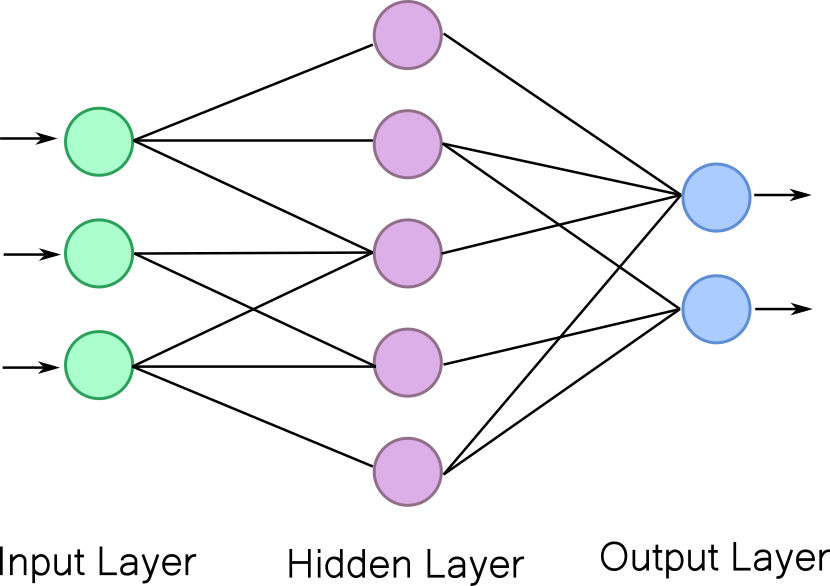
\includegraphics[width=0.6\linewidth]{ffnn}
    	\caption{Abstract structure of a feed-forward neural network. A real network will have many more layers and a lot more neurons per layer. Own figure.}
    	\label{fig:ffnn}
    \end{minipage}
	\hfill
	\begin{minipage}[t]{0.45\textwidth}
		\centering
		\begin{tikzpicture}[scale=0.5, transform shape]
  			\begin{axis}[scale only axis,
    					axis lines=middle,
    					inner axis line style={=>},
    					xlabel={},
    					ylabel={},
    					ytick={-1,-0.5,...,1},
    					xtick={-1,-0.5,...,1},
    					ymin=-1,
    					ymax=1,
    					xmin=-1,
    					xmax=1
  						] 
    			\addplot [mark=none,  blue,   ultra thick] {max(0, x)}; 
  			\end{axis}
		\end{tikzpicture}
    	\caption{Visualization of the ReLU activation function. Own figure.}
    	\label{fig:relu}
    \end{minipage}
\end{figure} 

\section{Neural Networks}

The following sections dissect the individual components of a neural network and explain concepts and procedures.

\subsection{Neuron}

A \textit{Neuron} is the smallest unit of a neural network and is essentially what the network is made up of. It computes the linear function 

\begin{align}
y = \sum\limits_{i=0}^kw_ix_i + b
\end{align}

where $w_i$ is the weight for the $i$-th input $x_i$ and $b$ is a bias. The weights and the bias are the values that can be learned during the training process of the network (see Section \ref{section:network_training}). The output of a layer of neurons of a network is the vector $(y_0, \cdots, y_t)$, $y_j$ being the output of the $j$-th neuron. Those outputs then serve as inputs to the next layer, although not every output has to be used by every next neuron. To prevent the network from collapsing into a single linear classifier and thus to increase the expressivity of the network, the output of a neuron is put into a non-linear so-called activation function. Although many different activation functions exist, most popular is the one called \textit{Rectified Linear Unit (\gls{relu})}, which was first presented by Jarrett et al. in \cite{relu}. The function is exemplarily visualized in \fig \ref{fig:relu} and is calculated as

\begin{align}
f(x) = max(0, x)
\end{align} 

\subsection{Feed-Forward Neural Network}

A \textit{Feed-Forward Neural Network} is a network consisting of layers of neurons. The first layer is called the input layer. Those are the neurons that receive the data that the network is supposed to process. The last layer is called the output layer. The output of the neural network depends on the design implied by the use case. It can be object coordinates like in our case, class probabilities in classification tasks or any other real-valued output. The intermediate layers are called hidden layers. Their number can grow to over a hundred in modern networks \cite{resnet}, thus the name deep neural networks and deep learning. All layers can have different numbers of neurons and connections to previous layers. A schematic overview over the structure of a neural network can be seen in \fig \ref{fig:ffnn}. A neural network can be seen as the function $y=f(x,\theta)$, where $\theta$ are the weights and biases of the neurons and some other parameters an $y$ is the output of the network.

\subsection{Convolutional Neural Networks}

\begin{figure}[!tbp]
	\centering
	\begin{subfigure}[t]{0.45\textwidth}
		\centering
    	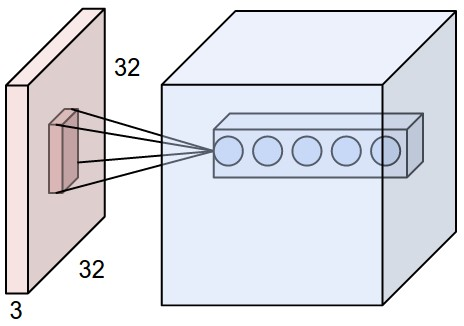
\includegraphics[width=0.7\linewidth]{conv_layer}
    	\caption{Example convolutional layer. The input image has dimensions 32x32 and 3 channels. The blue volume is the actual convolutional layer with multiple filters.}
    	\label{fig:conv_layer}
	\end{subfigure}
	\hfill
	\begin{subfigure}[t]{0.5\textwidth}
		\centering
    	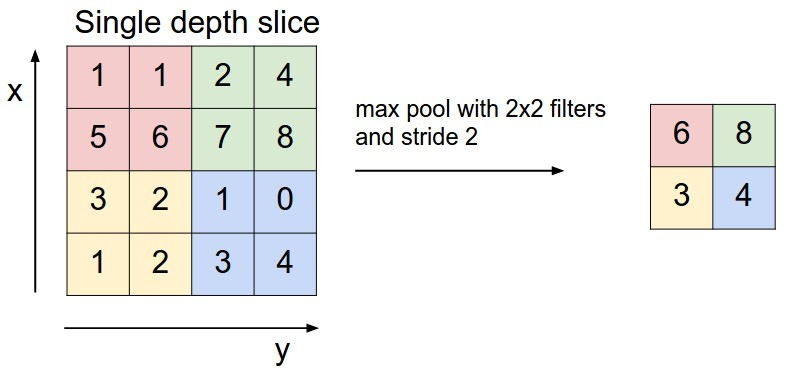
\includegraphics[width=0.9\linewidth]{pool_layer}
    	\caption{Example pooling layer with maximum as pooling operation.}
    	\label{fig:pool_layer}
	\end{subfigure}
	\caption{The two main layer types of a convolutional neural network.}
\end{figure} 

A \textit{Convolutional Neural Network (\gls{cnn})} describes a certain type of feed-forward neural network that consists of mainly two types of layers: \textit{Convolutional Layers} and \textit{Pooling Layers}. Normally, one or more convolutional layers are followed by a pooling layer. A convolutional layer convolves its input with a kernel which is moved along the input's dimensions. The kernel weights are shared, i.e. stay the same for the convolution of the whole input. \fig \ref{fig:conv_layer} shows the schematic of a convolutional layer. Each filter of the layer extends the output in the third dimension and has its own kernel. To reduce the size of the data a pooling layer can be added after the convolutional layer. This significantly speeds up computation and reduces the memory needed. It also reduces the number of parameters which helps to prevent the network from overfitting. An overfitted network performs well on the data it was trained on but does not generalize well, thus does not perform well on unseen data. Some architectures draw on a \textit{Fully-Connected Layer} as the last layer to perform the actual classification, etc. In such a layer every neuron is connected to every previous output. Convolutional neural networks are often used in computer vision tasks like image classification, instance segmentation and many more.

\subsection{Network training} \label{section:network_training}

When a network is created, usually its weights and biases are initialized to 0 or sampled randomly from a Gaussian distribution. To set the parameters to meaningful values that produce the desired output, the network has to be trained. We will now have a look at different techniques how to train a network.

\subsubsection{Error-Back Propagation} The predominant procedure to train a network is called \textit{Error-Back-Propagation} or \textit{Backpropagation}. To employ backpropagation, a differentiable but arbitrary loss function has to be defined. The loss function measures the error of the output of the network, e.g. by summing up the squared differences of the output and the objective output. The network is then applied to a training example in the so-called forward pass. Next, the loss function is derived with respect to each network weight using the chain rule of calculus. The derivative, the computed and the desired output together yield the change, also called delta, to be applied to the weights of the neuron. This delta is then propagated backwards through the net to calculate the deltas of the layers in between, again using the chain rule. After the deltas for all neurons have been computed, the weights are updated according to an update rule (see next paragraph). 

\subsubsection{Optimization} There exist many different patterns how to update the network weights after obtaining the detlas. The \textit{Stochastic Gradient Descent (\gls{sgd})} multiplies the delta by a learning rate and subtracts it from the weight. To ensure convergence, often the learning rate is decreased over time. A more elaborate method is the \textit{Adaptive Moment Optimization (Adam)} \cite{adam} which computes adaptive learning rates for each parameter. Here, an exponentially decaying average over past gradients as well as an exponentially decaying average over the past squared gradients serve to increase the learning rate in case of small gradients and decrease the learning rate in case of large gradients. Both averages are stored for the next iteration. Adam has greatly benefited the training process and proven to decrease computation time by finding local minima faster than \gls{sgd}. Other optimization procedures exist as well but will not be covered here.
	
\subsubsection{Regularization} Regularization can mean various things for neural networks. In general, its purpose is to keep the network from overfitting. Ian Goodfellow defined it in \cite{goodfellow} as any modification that reduces the generalization error but not the training error. Many network architectures regularize the net by adding a penalty term on the weights. Another possibility is to randomly deactivate a portion of the neurons to force the network to compensate the missing information, which is called \textit{Dropout}. \textit{Batchnormalization} helps the network generalize by subtracting the batch mean and batch standard deviation from the output of the previous layer. A batch is a subset of the input data which the network is trained with. This technique is often employed when the underlying machine can't fit the whole dataset in memory and because the network typically trains faster this way. To keep \gls{sgd} or other optimizers from reversing the covariance shift performed by batchnormalization the two parameters \textit{beta} and \textit{gamma} of such a layer are trainable.

\section{6D Pose Estimation}

\begin{figure}[!tbp]
	\centering
	\begin{subfigure}[t]{0.3\textwidth}
		\centering
    	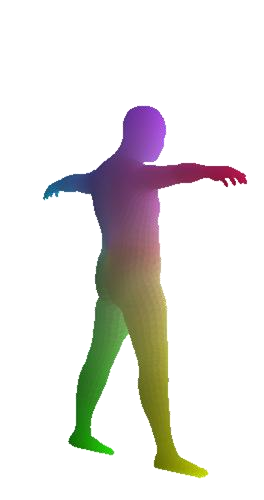
\includegraphics[width=0.45\linewidth]{human_object_coordinates}
    	\caption{The object coordinate representation of a human. Image from \cite{tsharp}.}
    	\label{fig:human_object_coordinates}
	\end{subfigure}
	\begin{subfigure}[t]{0.3\textwidth}
		\centering
    	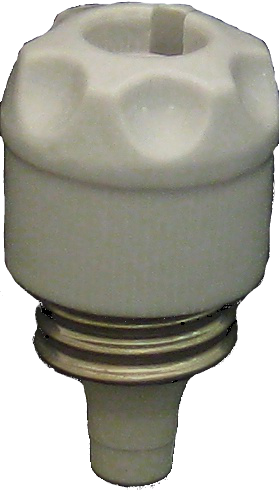
\includegraphics[width=0.45\linewidth]{tless_object}
    	\caption{An example object from the T-Less dataset. Image from \cite{tless}.}
    	\label{fig:tless_object}
	\end{subfigure}
	\begin{subfigure}[t]{0.3\textwidth}
		\centering
    	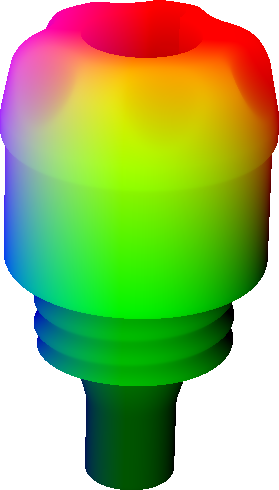
\includegraphics[width=0.45\linewidth]{tless_object_coordinates}
    	\caption{And the corresponding rendered 3D object coordinates (scaled for visualization). Own image.}
    	\label{fig:tless_object_coordinates}
	\end{subfigure}
	\caption{Example 3D coordinate representations.}
\end{figure} 

\textit{6D pose estimation} is a central task in the computer vision community. The goal is to retrieve an object's translation and rotation from an image, relative to the camera. \textit{6}D refers to the \textit{6-Degrees-of-Freedom (6-\gls{dof})}, i.e. the 6 free parameters of the \textit{3}D translation and \textit{3}D rotation. The field of application ranges from medical imaging, robotics, augmented reality, and many others. Different systems provide different accuracy. Setups using two cameras for stereo vision or depth information in addition to colors achieve good results. As endoscopes usually do not provide depth information or stereo vision, this work focuses on pose estimation using RGB-only images.

There are different possible ways to estimate the pose with learning-based approaches. The 6 parameters can be predicted directly or an intermediate representation can be used for pose computation. Predicting the parameters directly can be problematic, as the output of the neural network underlies noise and there is no possibility to verify or improve the pose afterwards. This is the reason why this work employs a network with a dense output, i.e. one output  for each pixel. The output for a pixel are the 3D coordinates on the object. Each subset of object coordinates leads to a certain pose. Some coordinates may contradict a pose and therefore the pose with the least contradictions is chosen as the best one. The next section will introduce this concept of so-called object coordinates in depth.

\subsection{Object Coordinate Regression} \label{objectcoordinates}

\begin{figure}[!tbp]
	\centering
    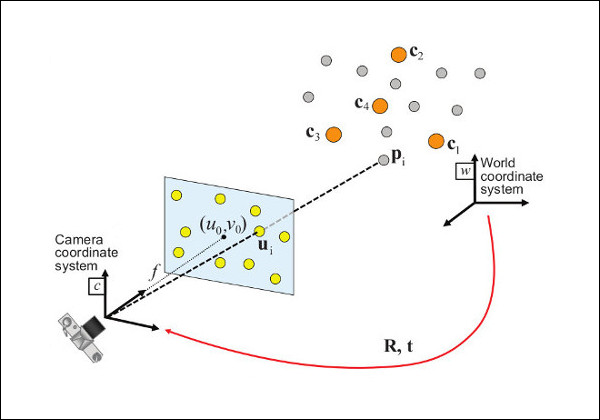
\includegraphics[width=0.45\linewidth]{pnp}
    \caption{The relationship between the camera, the 3D points and their projections on the screen using the rotation matrix $R$ and the translation vector $t$. Image from \cite{opencv_pnp}.}
    	\label{fig:pnp}
\end{figure} 

Tayler et al. first used object coordinates in \cite{tsharp}. Instead of directly predicting the location of joints or limbs of the human body they computed for each pixel the corresponding 3D location on the person (see \fig \ref{fig:human_object_coordinates}). The idea can be transfered to objects of any kind. \fig \ref{fig:tless_object} shows an example object from the T-Less dataset \cite{tless} and \fig \ref{fig:tless_object_coordinates} shows the corresponding rendered 3D object coordinates.


TODO: this is not entirely correct
The 3D coordinates and the respective 2D pixel locations on the image yield the \textit{Perspective-n-Point (\gls{pnp}) Problem}. That is, for a given pixel $p$ on the image and the corresponding 3D point $x$ (both in homogeneous coordinates), a pose consisting of the rotation matrix $R$ and the translation vector $t$ has to fulfill the following equation

\begin{align}
 p = K \ [ \ R \ | \ t \ ] \ x \label{eq:pose_projection}
\end{align} 

where $K$ is the camera matrix

\begin{align}
K = \begin{bmatrix}
f_x & s & c_x \\
0 & f_y & c_y \\
0 & 0 & 1 
\end{bmatrix}
\end{align}

which projects the 3D point transformed into the camera coordinate system on the 2D image plane. $s$ is a skew factor which is usually $0$, $(c_x, c_y)$ is the principal point, usually the center of the image and $f_x$ and $f_y$ is the focal lengths in $x$ and $y$ direction respectively. The values for those variables can vary when for example cropping the image. \fig \ref{fig:pnp} visualizes the relation of pixels and object coordinates. If equation \ref{eq:pose_projection} is overdetermined because there are more correspondences than variables it cannot be solved directly.

A method to solve the \gls{pnp} problem for many correspondences is to use the \textit{\gls{ransac} algorithm} \cite{ransac}. \gls{ransac} selects a model based on a subset of the dataset and evaluates it against the remaining data. This way the approximate best model is found iteratively. Algorithm \ref{algorithm:ransac} shows the outline of the \gls{ransac} algorithm for pose estimation. The energy function can be varied. It can for example be the number of inliers. Inliers are 3D points whose reprojected 2D location is within a certain area of the actual 2D location. Since \gls{ransac} is well known and employed in many different applications to estimate a model that fits a dataset best, we use it in this work to compute the pose. The implementation that is used is the one incorporated into the \textit{solvePnPRansac} method of the \textit{OpenCV} \cite{opencv} framework. 

\begin{algorithm}
\caption{RANSAC} \label{algorithm:ransac}
\begin{algorithmic} 
\REQUIRE Set of 3D points
\REQUIRE Set of corresponding 2D points
\REQUIRE Number of iterations $i$
\REQUIRE An energy function to score the pose hypothesis $E$
\STATE Set current energy $e=0$
\STATE Set current best pose hypothesis $h$ to $null$
\FOR{$1 ... i$}
\STATE Select a subset of corresponding points to compute pose $H$
\STATE Compute energy of the pose $e'=E(H)$
\IF{$e' > e$}
\STATE Store pose $H$ as current best in $h$
\STATE Set $e = e'$
\ENDIF
\ENDFOR
\RETURN Best pose $h$
\end{algorithmic}
\end{algorithm}
\chapter{Related Work}

In the following section, we investigate the current state of research on 6D pose estimation. The chapter starts with an excerpt of non-learning-based methods. We then present more recent, learning-based works with emphasis on active learning and fine-tuning of neural networks.

\section{Research on 6D Pose Estimation}

Pose estimation has become an increasingly interesting problem with the advent of robots in production and the area of virtual and augmented reality \cite{bb8}. Research before the rise of learning-based methods focused on manual feature extraction, divided into the major groups of sparse, dense and template-based approaches. Nowadays scientists often employ learning-based techniques which offer higher accuracy.

\subsection{Non-Learning-Based}

Before the major breakthrough of deep learning in 2012 \cite{alexnet}, handcrafted feature-based approaches were common for 6D pose estimation \cite{ylecun}. A lot of research matches sparse characteristics detected in the image against a database that contains the related pose information. The works of \cite{dglowe1, dwagner} use keypoints as the discriminative feature and offer good accuracy on well-textured objects. Unfortunately they yield bad performance on poor-textured or texture-less objects, because in those cases detectors are unable to find stable keypoints or any at all. The methods presented in \cite{gklein,dglowe2,charris} identify edges in the image and use different techniques to obtain an initial pose guess based on them. The resulting pose is retrieved by iteratively refining the previous guess, by minimizing the distance of the projected and detected edges.
\nnewline
Template-based methods \cite{hinterstoisser1, hinterstoisser2, rioscabrera, csteger} use generated views of discrete viewopints on the object at different angles which are matched against the given image to retrieve the pose. This approach relies mainly on the shape of objects and thus works well for poor-textured or textureless objects. To cover many objects and a large pose range the number of templates of an object has to be increased though, which slows down prediction. Hashing the views to speed up the pose estimator reduces accuracy \cite{zhou}. Additionally, deformed or occluded objects decrease precision, as templates globally reason about the object's pose.
\nnewline
Some authors draw on additional views to improve accuracy. Stereo camers are used in \cite{kpauwels}. A second image from another angle implies depth information to a certain extend but involes the additional task of stereo matching. The sudden availability of cheap depth sensors, like the Kinect, gave rise to algorithms making use of RGB-D images. Multiple approaches are possible when incorporating depth to retrieve an object's pose. Voting schemes were employed in \cite{bdrost, salasmoreno} and achieved good. First, a reference point in the image is selected and paired with all other points. The point pair feature called pair then votes for a possible pose, if their distance and respective normals are contained in the global sparse model description. The pose with the most votes is deemed to be the optimal one.

\subsection{Learning-Based}

Methods that learn information about objects - that is not explicitly modeled - started to outperform the previous techniques. There exist a vast literature for this task but we restrict our review to recent works that are most relevant to our approach.
\nnewline
Lai et al. use decision tress in \cite{klai}, which incorporate the semantic information of objects and their poses. Tom{\`{e}} et al. predict human poses from single RGB images in an end-to-end fashion \cite{dtome}. The system of \cite{azeng} relies on multi-view images and depth information and scored the 3rd and 4th place in the Amazon Picking Challenge 2016 \cite{apc}. A prominent example of the problem of camera localization, which is estimating the camera position in 3D space relative to the scene, is PoseNet \cite{posenet}. The underlying architecture of the employed neural network is based on GoogleNet, which was introduced in \cite{googlenet}. The CNN estimates the camera position from a single image in an end-to-end fashion and is fast, but, with an error of 50 centimeters in some cases, too inaccurate to reliably estimate poses of surgical tools.

\paragraph{BB8.}

The recently developed BB8 \cite{bb8}, which is an abbreviation for the 8 corners of the bounding-boxes of objects, is the result of the work of Rad and Lepetit that operates on RGB-only images. Instead of regressing the pose of an object with object coordinates like \cite{brachmann1}, they let a deep neural network estimate the object segmentations first and then predict the 2D locations of the 3D corners of the object's bounding box. 
\nnewline
\begin{figure}[!tbp]
	\centering
	\begin{subfigure}[b]{0.45\textwidth}
		\centering
    	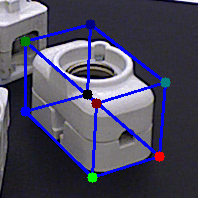
\includegraphics[width=0.45\linewidth]{bb8}
    	\caption{The control points of the object's bounding box.}
	\end{subfigure}
	\hfill
	\begin{subfigure}[b]{0.45\textwidth}
		\centering
    	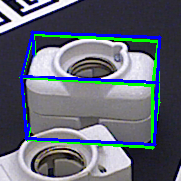
\includegraphics[width=0.45\linewidth]{bb8_prediction}
    	\caption{The final estimated pose. Green is the groundtruth.}
	\end{subfigure}
	\caption{Example images displaying the functioning of BB8. Images taken from \cite{bb8}.}
\end{figure}
Despite its differences to \cite{brachmann1}, the object's position is not predicted directly either, but instead regressed by solving the perspective-n-point (PnP) problem of the correspondences of the corners of the object's bounding box and the projected 2D locations of the corners predicted by the network. The architecture of the first and second net is based on VGG \cite{vgg} respectively but with the last layer cut off and replaced by a fully connected layer which is fine-tuned. 
\nnewline
The first network, which segments the image, helps estimating the pose of the object in a way that the second network positions its window at the center of the segmentation and predicts the pose. The pose prediction works by estimating the 2D locations of the 3D corners of the object's bounding box. The network reasons globally about the object by not moving the window containing the object during training and prediction. The authors argue that patch-based pose estimators are typically very noisy, and hence require a robust optimization scheme, like RANSAC. 
\nnewline
Unfortunately, BB8's take on pose estimation fails on symmetric objects, when implemented directly as described above. To address this problem, the authors first estimate the rotational angle of the object, and mirror the image if necessary. This way, a CNN can be trained only on a certain range of the angle of the pose.
\nnewline
The proposed method offers good performance and can compete with and partly surpasses state-of-the-art research. Yet, object coordinates provide high accuracy too and due to the assumption of the author of this work, that the often merely patch-wise visibility of the surgical instruments calls for a non-global reasoning design BB8 is followed any further in this work.

\paragraph{SSD-6D.}

The system presented in \cite{ssd-6d} is based on the work in \cite{ssd}, called Single-Shot Multibox Detector, or short SSD. Their take on 6D pose estimation is especially alluring, as the authors train the network exclusively on synthetic data. A positive outcome would imply that the lack of already annotated datasets for 6D pose estimation could be overcome by generating data for network training. 
\nnewline
Kehl et al. let the network estimate the probability of a discrete viewpoint on the object. Those viewpoints are sampled equidistant alongside a predefined degree step-size to represent all possible poses of the objects. This view estimate, combined with an estimate on the rotation, is used to generate pose predictions. 
\nnewline
\begin{figure}[!tbp]
	\centering
	\begin{subfigure}[b]{0.3\textwidth}
		\centering
    	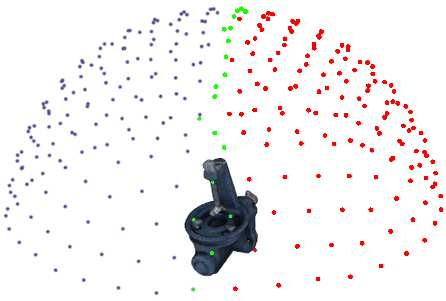
\includegraphics[width=\linewidth]{ssd_6d_sphere}
    	\caption{An exampe of a discrete distribution of viewpoints on an object.}
	\end{subfigure}
	\hfill
	\begin{subfigure}[b]{0.6\textwidth}
		\centering
    	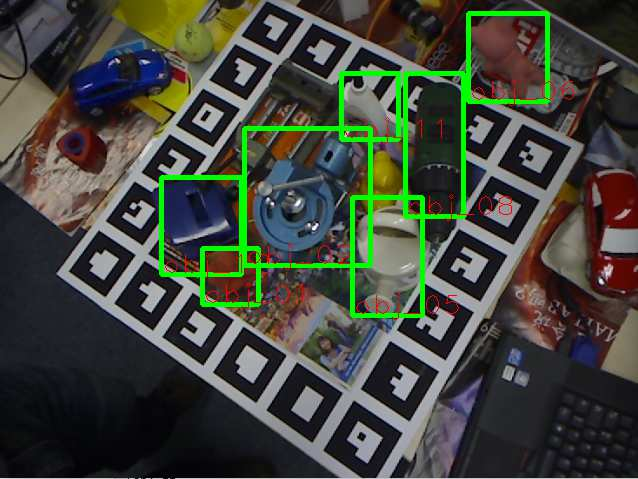
\includegraphics[width=0.45\linewidth]{ssd_6d_bb}
    	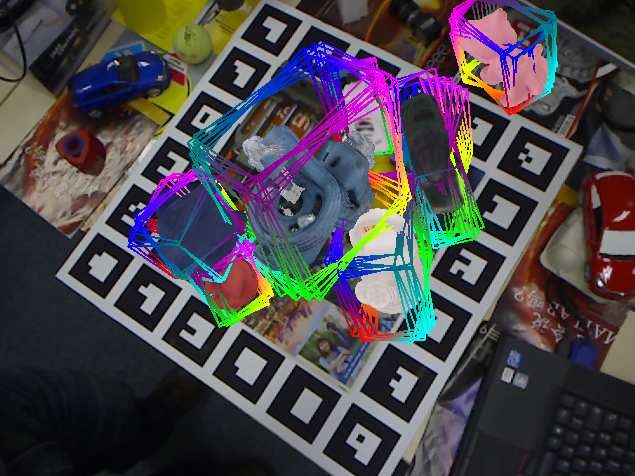
\includegraphics[width=0.45\linewidth]{ssd_6d_pose}
    	\caption{Left image: An example for bounding boxes found by the SSD-6D network. Right image: The most confident views and rotations for those boxes.}
	\end{subfigure}
	\caption{Example images displaying the functioning of SSD-6D. Images taken from \cite{ssd-6d}}
\end{figure}
The SSD-inspired network architecture produces feature maps that are convolved to predict the class, 2D bounding box, viewpoint scores and in-plane rotation of an object. The network is trained entirely on images from the MS COCO dataset \cite{mscoco} with the objects to be detected rendered into with arbitrary translations and rotations. For each transformation, the network is given the closest discrete viewpoint, in-plane rotation and the tightest bounding box as a regression target.
\nnewline
The author's reasoning, that their approach on pose estimation is a more natural one than pose regression stands to reason, as a human learns what an object looks like by viewing it from different angles. Nevertheless, the network produces rather inaccurate initial results.  To remedy this drawback, an optimization scheme extracts 3D contour points from the rendered hypothesis and minimizes the distance to the detected 2 locations of the points on the image. 
\nnewline
Since the neural network alone performs less well compared to \cite{brachmann1} or \cite{bb8} and the approach requires an optimization process, which could also be applied to the two mentioned works, it is not investigated further. 

\paragraph{Kurmann et al.}

The work of \cite{kurmann} estimates poses of surgical instruments in minimally invasive surgery. Similarly to object coordinate regression, Kurmann et al. develop a system that produces probabilities of the presence of an object but not in a dense way but instead only for the joints of the tools. Their design draws on a scene model which holds how many tools can be visible at most, what tools are currently visible and what parts of those tools.
\nnewline 
The authors of that paper argue that the common two-stage pipeline for 6D pose estimation, that consists of object detection and then pose estimation, results in a more complicated design, and criticize that a sliding window approach might miss very small or very large instruments, i.e. advocate a global reasoning design.
\nnewline
The architecture of the employed network is based on the U-Net developed by the authors of \cite{oronneberger}, and trained by optimizing the cross-entropy derived from the scene model described earlier. The network architecture of U-Net is extended by a fully connected layer that is trained to predict the probabilities of the instruments.
\nnewline
The results of the design look promising and run time per image is around $100 ms$, enabling it to be deployed as a real-time solution. Conversely, mainly literature of the biomedical imaging was considered and compared, disregarding research work in other areas on pose estimation.

\subsection{Learning-Based: Object Coordinate Regression}

An interesting section of learning-based pose estimation are the works employing the method of so-called object coordinate regression (see Section \ref{objectcoordinates}). The idea is based on \cite{tsharp} and \cite{firstcoordinateregression}. The first used it to estimate the pose of a human body, the latter to regress the cameras position in a scene retrieved from a single RGB-D image.
\nnewline
Brachmann et al. achieved record-breaking results in \cite{brachmann1} for texture-less objects and good performance in general. The authors based their work on forests instead of trees to regress the object's pose. The forests are trained to jointly predict the probability of object instances as well as the object coordinate probability for a given pixel. The output of the forest is processed in an energy function that imposes an energy minimization problem to regress the object's pose. A RANSAC-like scheme then iteratively refines the pose.
\nnewline
In \cite{brachmann2}, Brachmann et al. adjusted their pipeline from \cite{brachmann1} to work with RGB-only images. To reduce uncertainty in the object instance and coordinate predictions they incorporate an auto-context framework and marginalize the object coordinates over the depth information to cope with the missing fourth channel. The presented system outperforms Brachmann et al.'s previous work but is still based on forests. 
\nnewline
Krull et al. elaborated \cite{brachmann1} by replacing the energy function by a CNN \cite{akrull}. They were able to further improve the performance and transfer object coordinate regression to modern deep neural networks. The system called PoseAgent fuses regression forests and CNNs \cite{poseagent}. The regression forest outputs pose hypotheses that the CNN then refines. Krull et al. are able to achieve state-of-the-art results and improve resource utilization. Although \cite{trees-vs-cnn} finds, that random forests partly offer a slightly superior performance, neural networks can compete and are therefore the focus of this work.

\paragraph{Pertsch.}

Although \cite{pertsch} also works with RGB-D images, we present his work here as the author proposes an easy extension to adapt the entire process to RGB-only images and presents promising results. The work by Pertsch is based on \cite{brachmann1}, i.e. uses object coordinates  (see section \ref{objectcoordinates}), but replaces the random forest with a CNN. The developed pose estimation pipeline relies on three steps. The first one segments the image, the second regresses the object coordinates, and the last one evaluates pose hypotheses. 
\nnewline
We don't to go into detail into the first operation of the pipeline as our training and test data already includes segmentations and we can hence omit it completely. The second stage consists of a multilayer CNN-architecture to predict the object coordinates. The architecture consists of an encoder-decoder multilayer network. Inspired by \cite{oronneberger}, the author assimilates skip-layer connections. The network computes object coordinates for each pixel of the previously computed segmentation. Pertsch employs a RANSAC-scheme to improve the quality of the predicted final pose. Two different methods to retrieve the pose are presented in the work, one relying on the energy function introduced in \cite{brachmann1} but in an altered version, and one procedure solely drawing on RGB information without the additional depth of a sensor. The latter, which is more relevant for us as we do not have any depth readings, is based on the earlier presented \cite{brachmann2}. 
\nnewline
Instead of penalizing depth divergences of the rendered depth from the estimated pose and the sensor readings, the number of pixels whose reprojection error is greater than a certain threshold is minimized iteratively by the RANSAC algorithm. This allows for the RGB-only extension that the author suggests but does not elaborate in detail. Without depth the pose regression becomse a PnP problem, that can be solved by a PnP solver which takes at  four 3D-2D point correspondences as input. We pursue a similar approach in our work which differs in architecture of the network, the steps of the pipeline and the input data. But the general ideas of \cite{pertsch} and especially \cite{brachmann1} are adopted and further complemented with current research and active and incremental learning.

\section{Research on Active and Online Learning}

Online learning considers how to incorporate new available data into a trained model or neural network. Active learning is the field of selecting data that a human should annotate manually, because the model does not perform well on it. The literature survey \cite{activesurvey} gives an overview over methods developed before 2011. Wang and Shang, the authors of \cite{dwang}, might be among the first to incorporate active learning into deep learning though, according to \cite{zhou}. In \cite{hyperspectral}, Al Rahhal et al. apply a similar idea to hyperspectral image classification, a task that shares the foibles to be tedious and time-consuming with biomedical image annotation. The authors developed an active selection paradigm to electrocardiogram classification. 

\paragraph{Zhou et al.}

In \cite{zhou}, Zhou et al. describe a novel process of actively demanding data to be annotated to improve the network quality and apply the newly available data in an incremental manner. They focus on this area because annotating biomedical images is still a time-consuming task that requires a lot of expertise and skill.
\nnewline
Opposed to retraining from scratch, the network is fine-tuned by an incremental tuning algorithm. According to the authors, researchers have shown that this offers superior performance. In contrast to our task, the authors want to achieve improvements on image classification and frame detection, but work on biomedical images nonetheless.
\nnewline
\begin{figure}[!tbp]
	\centering
    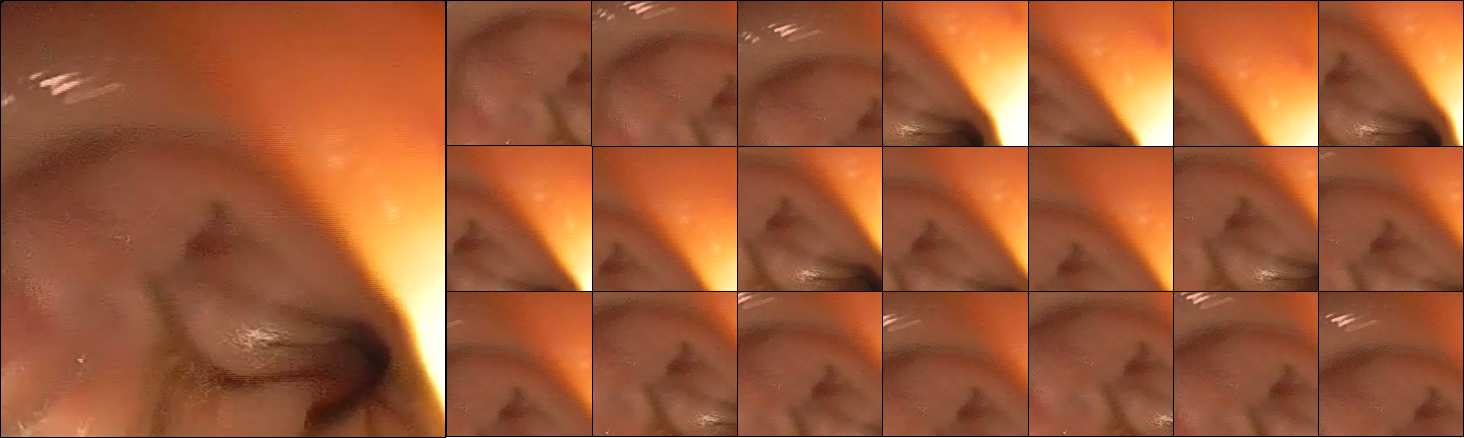
\includegraphics[width=0.7\linewidth]{fine_tuning}
	\caption{A candidate (left) and the patches generated sharing the same label. \cite{zhou}}
	\label{fig:zhou}
\end{figure}
Computer-aided-diagnosis (CAD) systems usually provide a candidate generator, which can quickly produce candidates, including true and false positives, to train with. Through data augmentation the learner can be made more robust to unforeseen situations. For this, numerous patches sharing the same label are generated from the candidate, as can be seen in Figure \ref{fig:zhou}, an presented to the classifier. 
\nnewline
The active selection process of candidates requires a measure of the worthiness of a candidate. To achieve this, the entropy and diversity of patches are calculated using the network's predictions for the patches of a candidate. Entropy is the negative log-likelihood of the network's prediction, whereas diversity captures how much patches of a candidate contradict, as they should all share the same label. Candidates with contradicting patches or low entropy can be selected for manual annotation.
\nnewline
The procedure quickly improves the neural network's accuracy. Learning from scratch or random selection of next candidates are quickly  outperformed, as only around 20\% of manually annotated candidates are necessary to reach the same error rate with the presented procedure.
\nnewline
In our case, data augmentation is possible, as we can render synthetic images, but the unnatural lightning and shadowing might decrease the accuracy of the design. The question of how to find  a worthiness measure arises too, as we can't directly tell how sure a network is when predicting a pose. But it provides a good direction of how to approach active learning.

\paragraph{Liu \& Ferrari.}

\begin{figure}[!tbp]
	\centering
    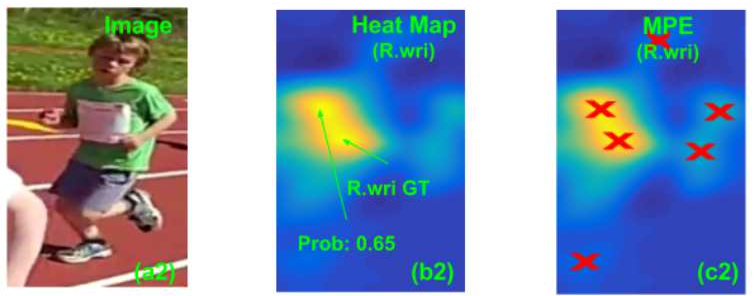
\includegraphics[width=0.6\linewidth]{human_pose_heatmap}
    \caption{An image of a human body, the corresponding heatmap as well as the result of the Multiple Peak Entropy (MPE). \cite{humanpose}}
    \label{fig:humanpose}
\end{figure}
In \cite{humanpose}, Liu and Ferrari describe new strategy for active learning for human pose estimation, a time-consuming task to produce groundtruth annotations for. Their key contributions consist of an uncertainty estimator for the joint predictions produced by a convolutional pose machine, and an annotation interface that reduces the time needed by a human annotator to click joints.
\nnewline
The active learning scheme incorporates influence and uncertainty cues. Influence cues consider images that are similar to other unlabeled images could propagate information. The uncertainty cues are measured by the uncertainty estimator. The estimator focuses on uncertain predictions, i.e. predictions with multiple weak peaks (multiple peak entropy). The functioning of the estimator can be seen in Figure \ref{fig:humanpose}. The final selection process then takes both cues into account when requesting an image to be manually annotated.
\nnewline
In addition, an interface is proposed that reduces the annotation time significantly. The system predicts a pose and segments the image around joints. The user can then right click anywhere in the segmentation to accept the estimated joint location or manually select it.
\nnewline
The results of \cite{humanpose} look auspicious, as a reduction in annotation time can be achieved through the interface and the selection process. Regrettably, it cannot be directly applied to our problem, as we need a problem-specific certainty estimator. But the idea of requesting similar images to be annotated might yield a performance gain, and similarly to the presented interface we present the user with an initial probable pose, too, to make only small corrections necessary.
\chapter{Program}
\chapter{Methods}
\chapter{Datasets}
%TODO provide example ground-truth object coordinates and predictions

\chapter{Experiments} \label{chapter:experiments}

The following section describes the setups of the experiments conducted with the neural network presented in chapter \ref{chapter:semi_automatic}. Due to the lack of existing annotated medical data the focus of the experiments is to ascertain a network design and mode of operation that compensate this as best as possible. First, we test the different network architectures that were described in section \ref{section:network_variations} using the same parameters. We then choose the best architecture for further experiments, in which we evaluate the two different training schemes introduced in section \ref{section:modes_of_operation}: training from scratch and incremental training.

\section{Terminology}

\noindent\textbf{Hyper-Parameter.} \textit{Hyper-parameters} are the tunable parameters of a network. The number and kind of parameters varies with the used type of network architecture, optimizer, etc.

\section{Datasets}

\begin{figure}[!tbp]
	\centering
	\begin{subfigure}[t]{0.47\textwidth}
		\centering
    	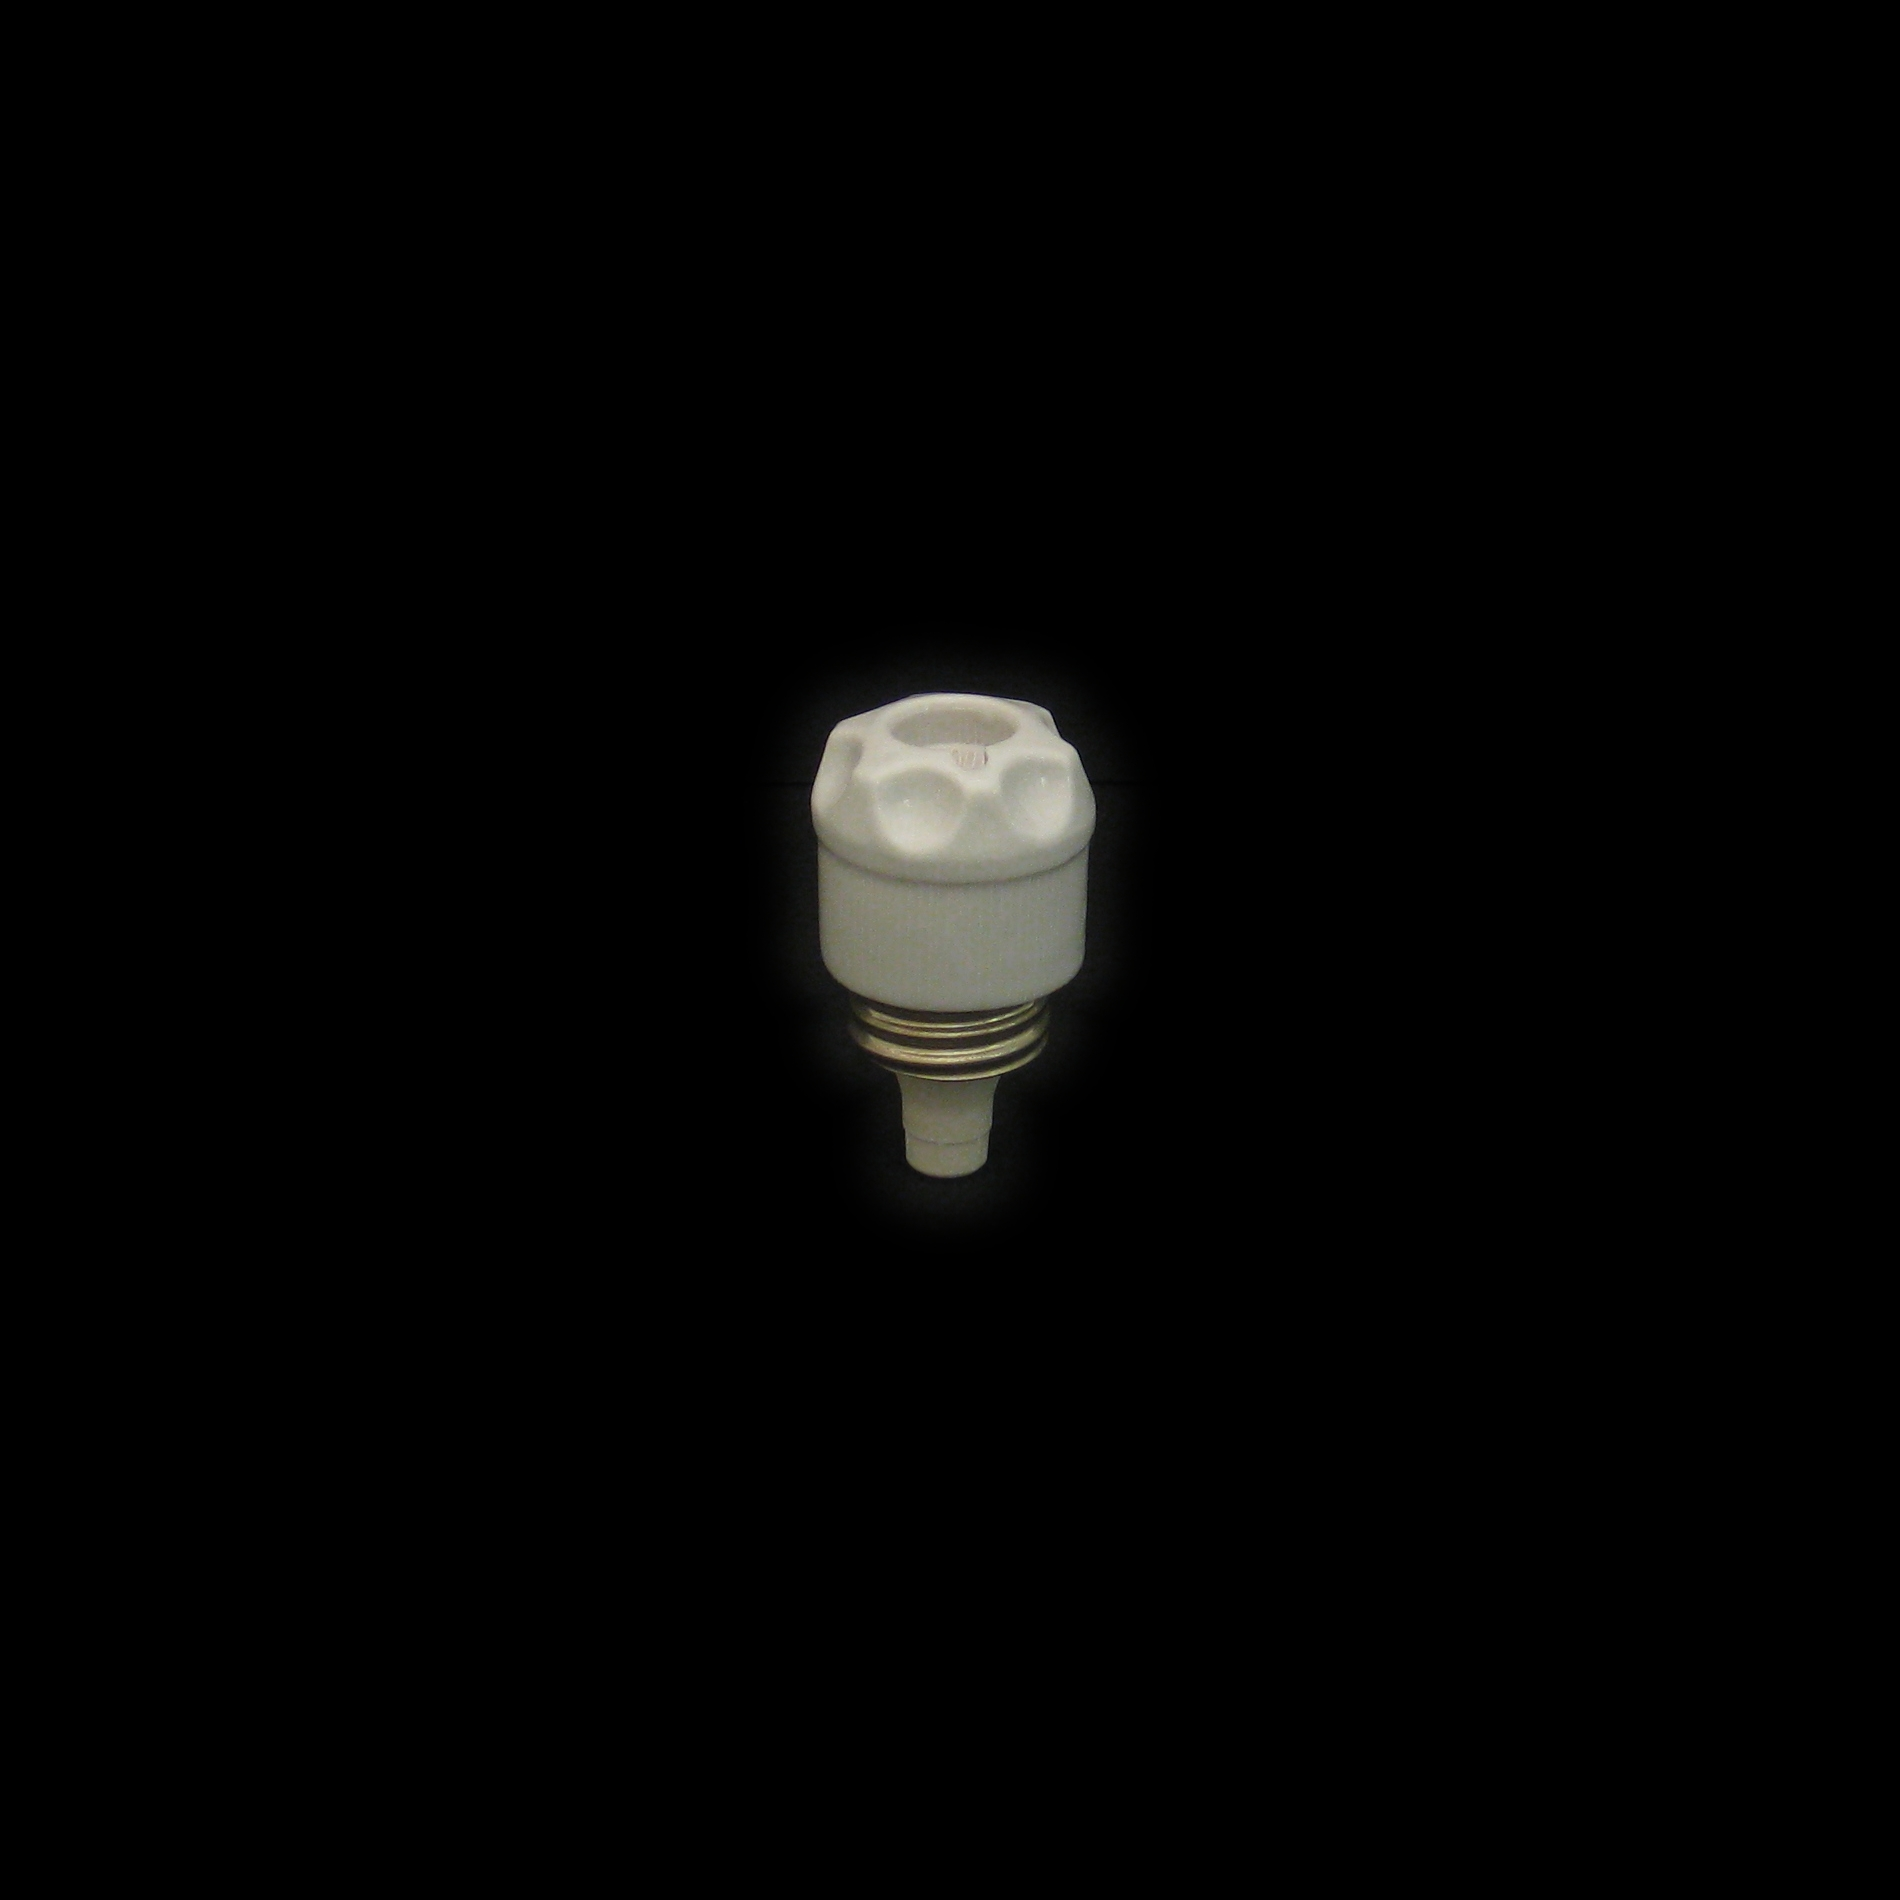
\includegraphics[width=0.6\linewidth]{tless_example_train}
    	\caption{An example frame from the training dataset of T-Less.}
    	\label{fig:tless_example_train}
	\end{subfigure}
	\hfill
	\begin{subfigure}[t]{0.47\textwidth}
		\centering
    	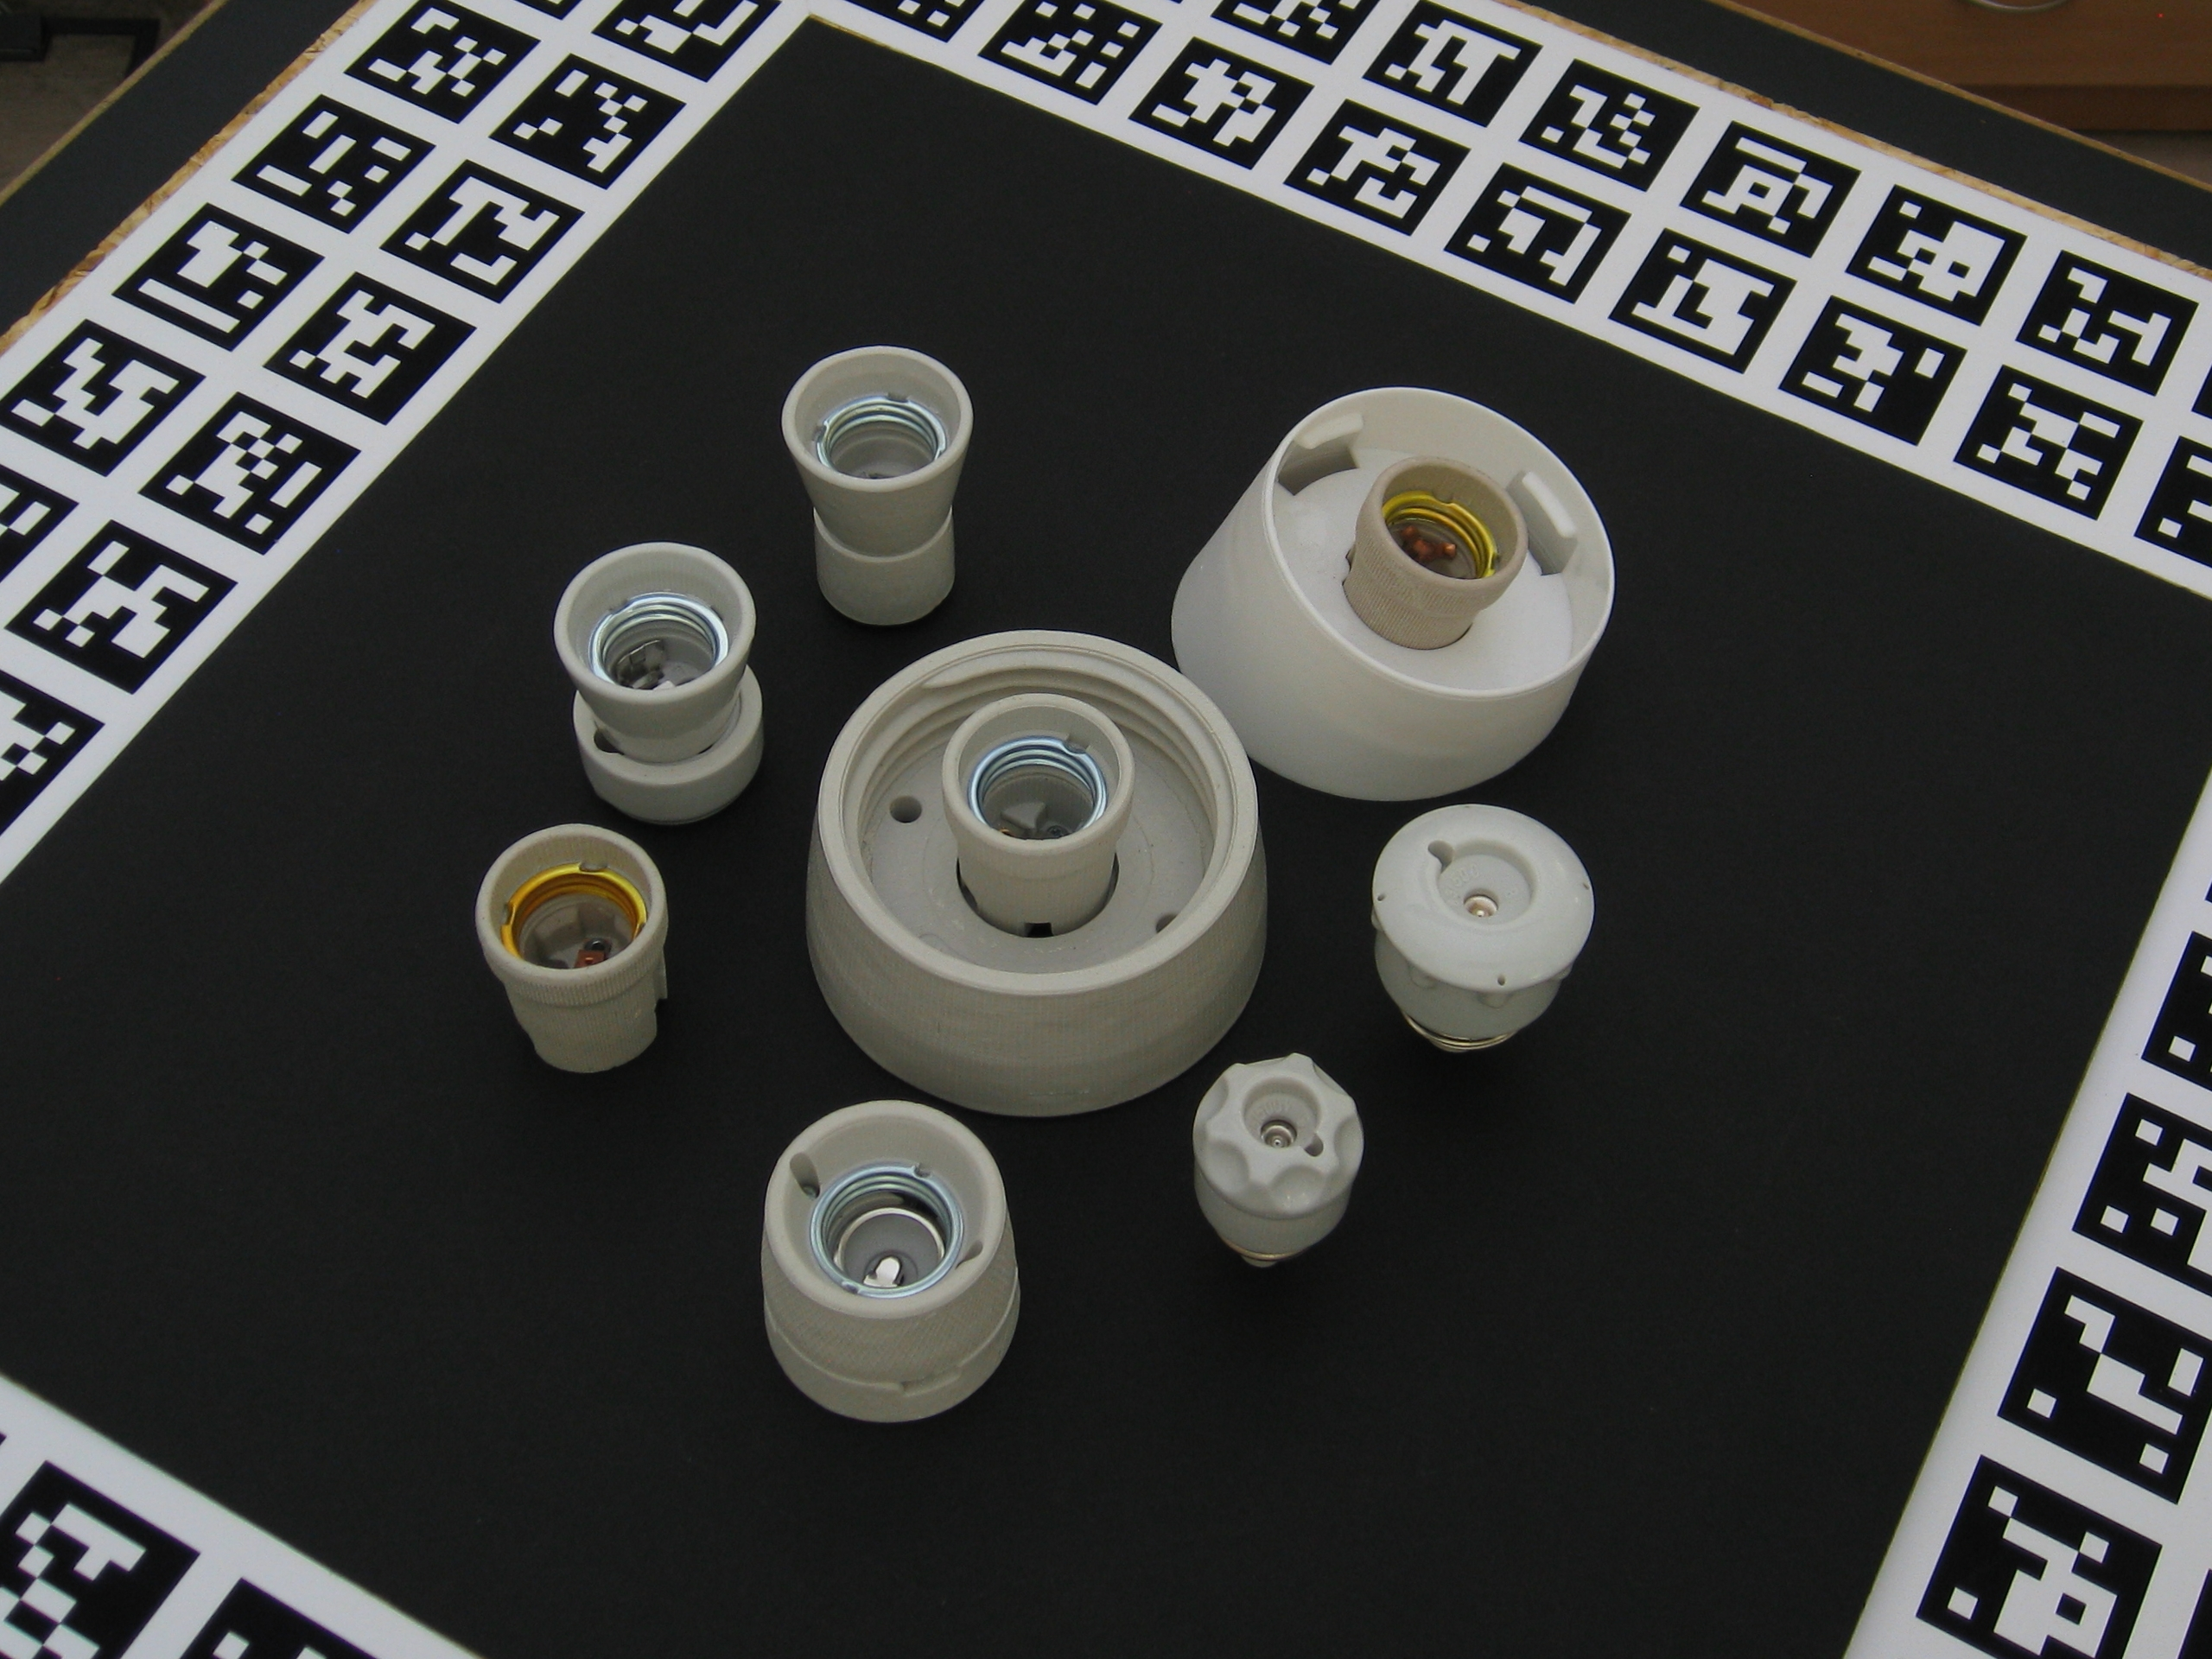
\includegraphics[width=0.7\linewidth]{tless_example_test}
    	\caption{An example frame from the test dataset of T-Less.}
    	\label{fig:tless_example_test}
	\end{subfigure}
	\caption{Example frames from the T-Less dataset \cite{tless}.}
	\label{fig:tless_examples}
\end{figure}

The initial intention to completely annotate the medical images provided at the beginning of the project turned out to be not feasible (see chapter \ref{chapter:manual_annotation}). Instead, we chose the T-Less dataset to conduct the experiments with. Its objects are mostly texture-less  and of rather small size making them similar to surgical tools. Next to many human pose estimation datasets, there exist some datasets of objects too, like \cite{next_view_dataset}, \cite{pracsys_dataset} and \cite{rigid_body_dataset}. But the objects of T-Less resemble surgical tools more than the objects of those datasets.

The T-Less dataset was released in 2017 by Hoda\v{n} et al. \cite{tless}. It contains the object models of 30 industry-relevant real world objects. Two versions exist: one mesh of the object that was manually reconstructed using CAD software and one that was produced from RGB-D images. The objects were captured using a Primsense CARMINE 1.09, a Microsoft Kinect v2 and a Canon IXUS 950 IS. We used the photos of the Canon camera due to their quality and we do not need depth information, which is also provided by the CARMINE sensor and the Kinect. There are 1296 images of each object in the training set of the dataset, sampled in 10 degree steps in elevation and 5 degree azimuth. 20 test scenes, consisting of 504 images each, exist as well. Those are photographs of cluttered scenes of different complexity, with sometimes more than 15 objects visible. All training and test images are annotated with the ground-truth poses of the visible objects. The authors also provided a tool set to render the objects at a given pose, etc. Fig. \ref{fig:tless_example_train} shows an example frame from the training set and fig. \ref{fig:tless_example_test} an example frame from the test set. The training images of the other objects look similar to the one shown. The dataset provides depth images, as well, but this is irrelevant to our setting.

\section{Data Preparation}

The \textit{T-Less} dataset does neither provide 3D object coordinates nor segmentation masks. This is the reason why we rendered both ourselves. The script is part of the network package. Because the 16-bit TIFF object coordinate ground-truth files used up too much disk space when in original size they were cropped to the relevant area by determining the smallest box around the segmentation pixels. The images and segmentation masks were cropped to the same area and the camera matrices adjusted accordingly. We used 16-bit TIFF files instead of 32-bit because we deemed the accuracy of 16-bit enough.

\section{Metric}

%TODO clarify using formulas

To be able to measure the accuracy of the different architectures and training techniques, we provide a metric to capture different aspects of the predictions. The error rate usually indicates the accuracy of the network. But in certain circumstances it makes sense to evaluate the predictions in a different way. One scenario that can occur is that the network predicts very inaccurate object coordinates at the border of the object's pixels. Since RANSAC eliminates outliers, the pose might not be much worse than a pose recovered from a prediction without outliers. The metric we defined measures the euclidean distance of the predicted and ground-truth coordinates, the number of inliers (pixels whose euclidean distance is below a certain threshold), as well as the angle error of the rotation and the euclidean distance of the translation of the recovered pose. This means, that the metric captures two error values based on the actual prediction and two based on the recovered pose. The script that we provide automatically calculates the mean but also outputs the median at 25, 50 and 75\% of the sorted error values. We assumed that the median at 50\% offers a good description of the accuracy of the network and used it to compare architectures and training setups.

\section{Training Experiments}

This section describes the configuration of the different training experiments. The chronological order of the experiments is reflected here. First, we compare the SGD and Adam optimizer in \ref{subsection:optimizers}. Then we evaluate the different architectures against each other in \ref{subsection:architectures}. Finally, asses the two training strategies training from scratch and incremental training in \ref{subsection:experiments_online_learning}. We conducted all experiments on the object model $01$ of the T-Less dataset. The image dimension was set to 500 pixels (for width and height), which is larger than the largest area covering an object in any image. All experiments were run using the training data of the object model $01$. For some experiments, we used only a subset of the available images (see Sections \ref{subsection:experiments_online_learning} and \ref{subsection:experiments_active_learning}) but we always split the data into 70\% training images and 30\% validation images. The axis labeled \textit{epochs} in loss graphs denotes the number of epochs the training was run for. Each epoch consisted of 1000 iterations in every experiment.

\begin{table}[]
\centering
\begin{tabular}{|l||lllll|}
\hline
Run                                                     & 1     & 2      & 3       & 4        & 5         \\ \hline \hline
\rowcolor{Gray}
Epochs                                                  & 30    & 45     & 55      & 65       & 70        \\
\begin{tabular}[c]{@{}l@{}}Learning\\ Rate\end{tabular} & 0.001 & 0.0001 & 0.00001 & 0.000001 & 0.0000001 \\  \hline
\end{tabular}
\caption{The configuration of the SGD optimizer used in the experiment to compare SGD and Adam.}\label{table:experiments_optimizers_sgd}
\end{table}

\subsection{Optimizers} \label{subsection:optimizers}  

\begin{figure}[!tbp]
	\centering
	\begin{subfigure}[t]{0.48\textwidth}
			\begin{tikzpicture}
  				\begin{axis}[cycle list name=tb, 
                 grid=both,
                 grid style={solid,gray!30!white},
                 axis lines=middle,
    			 xmin = 0,
    			 xmax = 100,
    			 ymin = 0,
    			 ymax = 3,
                 xlabel={epoch},
                 ylabel={loss},
                 x label style={at={(axis description cs:0.5,-0.1)},anchor=north},
                 y label style={at={(axis description cs:-0.1,.5)},rotate=90,anchor=south},]
      			\addplot[smooth,tb_color_1] table [x=Step, y=Value, col sep=comma] {experiments/model1/exp1_adam_l1/train_loss.csv};
      			\addplot[smooth,tb_color_2] table [x=Step, y=Value, col sep=comma] {experiments/model1/exp1_sgd/train_loss.csv};
      			\addlegendentry{Adam}
				\addlegendentry{SGD}
    			\end{axis}
			\end{tikzpicture}
		\caption{Training losses.}
	\end{subfigure}
	\hfill
	\begin{subfigure}[t]{0.48\textwidth}
			\begin{tikzpicture}
  				\begin{axis}[cycle list name=tb, 
                 grid=both,
                 grid style={solid,gray!30!white},
                 axis lines=middle,
    			 xmin = 0,
    			 xmax = 100,
    			 ymin = 0,
    			 ymax = 3,
                 xlabel={epoch},
                 ylabel={loss},
                 x label style={at={(axis description cs:0.5,-0.1)},anchor=north},
                 y label style={at={(axis description cs:-0.1,.5)},rotate=90,anchor=south},]
      			\addplot[smooth,tb_color_1] table [x=Step, y=Value, col sep=comma] {experiments/model1/exp1_adam_l1/val_loss.csv};
      			\addplot[smooth,tb_color_2] table [x=Step, y=Value, col sep=comma] {experiments/model1/exp1_sgd/val_loss.csv};
      			\addlegendentry{Adam}
				\addlegendentry{SGD}
    			\end{axis}
			\end{tikzpicture}
		\caption{Validation losses.}
	\end{subfigure}
	\caption{Training and validation losses of Adam and SGD used to train architecture 1. The plot is cropped on the $y$-axis to enhance the differences.}
	\label{fig:experiments_adam_sgd_loss}
\end{figure} 

To obtain the best optimizer for further experiments, we compared SGD and Adam using the first architecture we constructed. This architecture consists of 23 layers and has a receptive field-size of 99. The hyper-parameters $\beta_1$ and $\beta_2$ of the Adam optimizer were left at the default values set by Keras, which are $0.9$ and $0.999$, respectively. The more complex configuration of the SGD optimizer is given in Table \ref{table:experiments_optimizers_sgd}. Fig. \ref{fig:experiments_adam_sgd_loss} shows the loss of both experiments during training. The SGD optimizer profits from the reduction of the learning rate around step 30, visible as the small step in the training loss. This could imply that further tuning of the training parameters of SGD could lead to better results than the displayed ones. But since the Adam optimizer does not need manual fine-tuning of its hyper-parameters and performs visibly better than SGD, we chose Adam as the optimizer for all following experiments. We based our conclusion that Adam is the superior optimizer for our network solely on the loss values. Since we trained the same network architecture twice and only varied the optimizers, better error rates mean better overall results.

\subsection{Loss Functions}

\begin{table}[]
\centering
\begin{tabular}{|l||llll|}
\hline 
 Loss  & \begin{tabular}[c]{@{}l@{}}Object Coordinate\\ Error\end{tabular} & Inliers & Angle Error & Distance Error \\ \hline \hline \rowcolor{Gray}
L1 & 0.3413                                                            & 1738    & 0.0281      & 4.5574         \\
L2 & 0.8188                                                            & 1617    & 0.1090      & 8.3138 \\ \hline   
\end{tabular}
\caption{The metrics of the experiments comparing the loss functions.}
\label{table:experiments_loss_functions}
\end{table}

%TODO maybe rewrite this "to prove our statment...." -> did we prove it???

To prove our statement that the L1 loss is more suitable than the L2 loss for our application, we conducted another training run using the L2 loss and compared it to the run using the L1 loss of the previous experiment. The loss function comparisons are depicted in \ref{fig:experiments_l1_l2_loss} but are omitted here, due to their limited comparability. To obtain the L2 loss, we removed taking the square root in computing the loss which naturally results in higher error rates. Table \ref{experiments_loss_functions} shows the metrics of the experiments with the different loss functions. The L1 loss offers clearly superior accuracy and is used in all further experiments.

\subsection{Architectures} \label{subsection:architectures}

%TODO table of training parameters -> different batch sizes etc

\begin{figure}[!tbp]
	\centering
	\begin{subfigure}[t]{0.48\textwidth}
			\begin{tikzpicture}
  				\begin{axis}[cycle list name=tb, 
                 grid=both,
                 grid style={solid,gray!30!white},
                 axis lines=middle,
                 xlabel={epoch},
                 ylabel={loss},
                 x label style={at={(axis description cs:0.5,-0.1)},anchor=north},
                 y label style={at={(axis description cs:-0.1,.5)},rotate=90,anchor=south},]
      			\addplot[smooth,tb_color_1] table [x=Step, y=Value, col sep=comma] {experiments/model1/exp1_adam_l1/train_loss.csv};
      			\addplot[smooth,tb_color_3] table [x=Step, y=Value, col sep=comma] {experiments/model3/exp1/train_loss.csv};
      			\addplot[smooth,tb_color_6] table [x=Step, y=Value, col sep=comma] {experiments/model6/exp1/train_loss.csv};
      			\addlegendentry{Architecture 1}
				\addlegendentry{Architecture 3}
				\addlegendentry{Architecture 6}
    			\end{axis}
			\end{tikzpicture}
		\caption{Training losses.}
	\end{subfigure}
	\hfill
	\begin{subfigure}[t]{0.48\textwidth}
			\begin{tikzpicture}
  				\begin{axis}[cycle list name=tb, 
                 grid=both,
                 grid style={solid,gray!30!white},
                 axis lines=middle,
                 xlabel={epoch},
                 ylabel={loss},
                 x label style={at={(axis description cs:0.5,-0.1)},anchor=north},
                 y label style={at={(axis description cs:-0.1,.5)},rotate=90,anchor=south},]
      			\addplot[smooth,tb_color_1] table [x=Step, y=Value, col sep=comma] {experiments/model1/exp1_adam_l1/val_loss.csv};
      			\addplot[smooth,tb_color_3] table [x=Step, y=Value, col sep=comma] {experiments/model3/exp1/val_loss.csv};
      			\addplot[smooth,tb_color_6] table [x=Step, y=Value, col sep=comma] {experiments/model6/exp1/val_loss.csv};
      			\addlegendentry{Architecture 1}
				\addlegendentry{Architecture 3}
				\addlegendentry{Architecture 6}
    			\end{axis}
			\end{tikzpicture}
		\caption{Validation losses.}
	\end{subfigure}
	\caption{Training and validation losses of the different architectures.}
	\label{fig:experiments_architectures_loss}
\end{figure} 

The experiments run on the different architectures were all performed using the Adam optimizer with the parameters mentioned in Section \ref{subsection:optimizers} and the L1 loss. The major difference between the experiments is the architecture itself. The training process were run for a different number of iterations because some architectures converged earlier than others. The different losses are displayed in fig. \ref{fig:experiments_architectures_loss}.

\subsection{Online Learning} \label{subsection:experiments_online_learning}

%TODO  Check if number of images in plot is correct
      			
\begin{figure}[!tbp]
	\centering
	\begin{subfigure}[t]{0.48\textwidth}
			\begin{tikzpicture}
  				\begin{axis}[cycle list name=tb, 
                 grid=both,
                 grid style={solid,gray!30!white},
                 axis lines=middle,
                 xlabel={epoch},
                 ylabel={loss},
                 x label style={at={(axis description cs:0.5,-0.1)},anchor=north},
                 y label style={at={(axis description cs:-0.1,.5)},rotate=90,anchor=south},]
      			\addplot[smooth,tb_color_1] table [x=Step, y=Value, col sep=comma] {experiments/model1/exp1_adam_l1/train_loss.csv};
      			\addplot[smooth,tb_color_2] table [x=Step, y=Value, col sep=comma] {experiments/model1/exp2/train_loss.csv};
      			\addplot[smooth,tb_color_3] table [x=Step, y=Value, col sep=comma] {experiments/model1/exp3/train_loss.csv};
      			\addplot[smooth,tb_color_4] table [x=Step, y=Value, col sep=comma] {experiments/model1/exp4/train_loss.csv};
      			\addplot[smooth,tb_color_5] table [x=Step, y=Value, col sep=comma] {experiments/model1/exp5/train_loss.csv};
      			\addplot[smooth,tb_color_6] table [x=Step, y=Value, col sep=comma] {experiments/model1/exp6/train_loss.csv};
      			\addlegendentry{All}
      			\addlegendentry{500}
				\addlegendentry{250}
				\addlegendentry{100}
				\addlegendentry{50}
				\addlegendentry{25}
    			\end{axis}
			\end{tikzpicture}
		\caption{Training losses.}
	\end{subfigure}
	\hfill
	\begin{subfigure}[t]{0.48\textwidth}
			\begin{tikzpicture}
  				\begin{axis}[cycle list name=tb, 
                 grid=both,
                 grid style={solid,gray!30!white},
                 axis lines=middle,
                 xlabel={epoch},
                 ylabel={loss},
                 x label style={at={(axis description cs:0.5,-0.1)},anchor=north},
                 y label style={at={(axis description cs:-0.1,.5)},rotate=90,anchor=south},]
      			\addplot[smooth,tb_color_1] table [x=Step, y=Value, col sep=comma] {experiments/model1/exp1_adam_l1/val_loss.csv};
      			\addplot[smooth,tb_color_2] table [x=Step, y=Value, col sep=comma] {experiments/model1/exp2/val_loss.csv};
      			\addplot[smooth,tb_color_3] table [x=Step, y=Value, col sep=comma] {experiments/model1/exp3/val_loss.csv};
      			\addplot[smooth,tb_color_4] table [x=Step, y=Value, col sep=comma] {experiments/model1/exp4/val_loss.csv};
      			\addplot[smooth,tb_color_5] table [x=Step, y=Value, col sep=comma] {experiments/model1/exp5/val_loss.csv};
      			\addplot[smooth,tb_color_6] table [x=Step, y=Value, col sep=comma] {experiments/model1/exp6/val_loss.csv};
      			\addlegendentry{All}
      			\addlegendentry{500}
				\addlegendentry{250}
				\addlegendentry{100}
				\addlegendentry{50}
				\addlegendentry{25}
    			\end{axis}
			\end{tikzpicture}
		\caption{Validation losses.}
	\end{subfigure}
	\caption{Training and validation losses of the experiments of training architecture \textbf{1} from scratch but not with all images. The keys are the number of images used in training.}
	\label{fig:experiments_online_sratch_loss}
\end{figure} 

% Nochmal zusammenfassen scratch vs inkrementell

\subsection{Active Learning} \label{subsection:experiments_active_learning}

% Training on one side only -> provide metric results -> training on bad images -> new metrics

\subsection{Runtime Analysis}

This section analyses the inference runtimes of the different architectures. Deeper networks need longer to perform training and an inference run on an image, which is reflected by table ...

\subsection{Limitations}

% No challenge yet, difficult to tell how good network is -> no baseline!

% T-Less dataset contains only unoccluded images

% This way of comparing training procedures is owned to the timeframe of this work -> maybe L2 works better for model 5, etc., we generalize from one model to all others

% Create metric for images that the network produces bad predictions for, e.g. reprojection error for contradicting object coordinates, difference between segmentation mask rendered using the predicted pose and the ground-truth segmentation mask -> was not possible because we couldn't annotate images of the Endovis dataset

% Maybe training - validation ratio should be more like 90 - 10

% Difficult to say how the network would perform on the Endovis dataset -> we don't know if the networks with larger receptive field-size predict based on the letters
\chapter{Discussion} \label{chapter:conclusions}

In this chapter we summarize to work presented on the previous pages. We also draw conclusions from the results and give a an outlook of possible research based on this work in the future.

\section{Summary}

\section{Future Work}

% Train neural network on actual medical images

% Train neural network for multiple images

\bibliographystyle{IEEEtran}
\bibliography{bibliography.bib}

\end{document}